

\documentclass[a4paper,12pt,Times]{article}
\usepackage{abakos}  %pacote com padrão da Abakos baseado no padrão da PUC

%%%%%%%%%%%%%%%%%%%%%%%%%%%
%Capa da revista
%%%%%%%%%%%%%%%%%%%%%%%%%%

%\setcounter{page}{80} %iniciar contador de pagina de valor especificado
\newcommand{\monog}{Análise introdutória à Dispositivos Lógicos Programáveis }
\newcommand{\monogES}{Introduction to Programmable Logic Devices}
\newcommand{\tipo}{Artigo }  % Especificar a seção tipo do trabalho: Artigo, Resumo, Tese, Dociê etc
\newcommand{\origem}{Brasil }
\newcommand{\editorial}{Belo Horizonte, p. 28-03, mar. 2022}  % p. xx-xx – páginas inicial-final do artigo
\newcommand{\lcc}{\scriptsize{Licença Creative Commons Attribution-NonCommercial-NoDerivs 3.0 Unported}}

%%%%%%%%%%%%%%%%%INFORMAÇÕES SOBRE AUTOR PRINCIPAL %%%%%%%%%%%%%%%%%%%%%%%%%%%%%%%
\newcommand{\AutorA}{Ricardo Henrique Guedes Furiati}
\newcommand{\funcaoA}{}
\newcommand{\emailA}{rfuriati@sga.pucminas.br}
\newcommand{\cursA}{Aluno de Ciência da Computação}

% 
% Definir macros para o nome da Instituição, da Faculdade, etc.
\newcommand{\univ}{Pontifícia Universidade Católica de Minas Gerais}

\newcommand{\keyword}[1]{\textsf{#1}}

\begin{document}
% %%%%%%%%%%%%%%%%%%%%%%%%%%%%%%%%%%
% %% Pagina de titulo
% %%%%%%%%%%%%%%%%%%%%%%%%%%%%%%%%%%

\begin{center}

\includegraphics[scale=0.2]{figuras/brasao.jpg} \\
PONTIFÍCIA UNIVERSIDADE CATÓLICA DE MINAS GERAIS \\
Instituto de Ciências Exatas e de Informática

% \vspace{1.0cm}

\end{center}

\vspace{0cm} {
 \singlespacing \Large{\monog \symbolfootnote[1]{Trabalho da Disciplina de Arquitetura de Computadores} \\ }
  \normalsize{\monogES}
 }
\vspace{1.0cm}

\begin{flushright}
\singlespacing 
\normalsize{\AutorA \footnote{\funcaoA \cursA, \origem -- \emailA . }} \\
\normalsize{\AutorB \footnote{\funcaoB \cursB, \origem -- \emailB . }} \\

\end{flushright}
\thispagestyle{empty}

\vspace{1.0cm}

\begin{abstract}
\noindent
O seguinte artigo visa expor alguns conceitos básicos relacionados à Dispositivos lógicos programáveis (PLC's), diferenciando modelos e aplicações. O desenvolviemento do artigo fundamenta-se num primeiro contato com dispositivos e aplicações de sistemas digitais, relacionando-se com a disciplina de arquitetura de computadores.
\\\textbf{\keyword{Palavras-chave: }} PLC. Sistemas Digitais. Circuitos Integrados.
\end{abstract}

%%%%%%%%%%%%%%%%%%%%%%%%%%%%%%%%%%%%%%%%%%%%%%%%%%%%%%%%%
 \newpage    %%%% CASO QUEIRA QUE O RESUMO FIQUE EM UMA PAGINA E O ABSTRACT EM OUTRA
\selectlanguage{english}
\begin{abstract}
\noindent
The present article aims to aproach some basic concepts related to Programmable Logic Devices (PLCs), by diferentiating its models and applications. The development of the article is based in the first contact with digital systems and its applications, with the focus on the topic of computer architecture.
\\\textbf{\keyword{Keywords: }} PLC. Digital Systems. Integrated Circuits.
\end{abstract}

\selectlanguage{brazilian}
 \onehalfspace  % espaçamento 1.5 entre linhas
 \setlength{\parindent}{1.25cm}

%%%%%%%%%%%%%%%%%%%%%%%%%%%%%%%%%%%%%%%%%%%%%%%%%
%% INICIO DO TEXTO
%%%%%%%%%%%%%%%%%%%%%%%%%%%%%%%%%%%%%%%%%%%%%%%%%


\section{\esp Introdução}

    Um Dispositivo Lógico Programável (Programable Logic device - PLD) corresponde a um circuito integrado que, inicialmente, não possui uma função fixa (do ponto de vista lógico) sendo esta definida de acordo com a sua aplicação, por meio da programação. O advento deste tipo de tecnologia nas últimas três décadas do século XX permitiu um avanço significativo na área de sistemas digitais, tendo em vista que PLC's são mais flexíveis que portas lógicas comumente utilizadas. Ao longo do tempo, com o avanço tecnológico, diversos tipos de dispositivos lógicos programáveis foram desenvolvidos e difundidos, possuindo diversos níveis de especialização e aplicabilidade.

\section{\esp Tipos de Dispositivos Lógicos Programáveis}

Dispositivos lógicos programáveis se diferenciam de diversas maneiras, sendo a aplicação do dispositivo e processo de fabricação as mais abrangentes, por definirem as principais características dos PLC's.

\subsection{\esp Application Specific IC (ASICs)}

Circuito Integrado de Aplicação Específica (ASICs) é caracterizado por ter um processo de fabricação que varia de acordo com as necessidades de cada projeto. Este tipo de circuito possui um alto custo e tempo de fabricação quando comparado aos demais, o que faz com que ele nao seja viável para projetos grandes. 

\subsection{\esp Application-specific standard parts (ASSP)}
Circuito Integrado para aplicação específica padrão corresponde a um tipo de ASIC, entratanto possui uso um pouco mais generalizado.


\subsection{\esp Simple PLD's (SPLD)}

Dispositivo Lógico Programável Simples (Simple PLD) é caracterizado como um circuito integrado de baixo custo e alto desempenho. Ao contrário dos ASICs podem ser aplicados em diversos tipos de projetos e podem compor outros circuitos integrados.

\subsection{\esp Complex Programmable Logic Device (CPLD)}

Dispositivo Lógico Programável Complexo (Complex PLD) corresponde a um circuito integrado formado por vários SPLD (Dispositivos lógicos programáveis simples), que ao se combinar executam operações lógicas com maior grau de complexidade.

\subsection{\esp System on Chip (SOC)}
Sistema em um Chip (SOC) corresponde a um circuito integrado que possui a capacidade de armazenar um sistema operacional ou sequência de comandos. Geralmente é utilizado para controlar outros circuitos integrados ou sistemas lógicos.

\subsection{\esp Field Programmable Gate Array (FPGA)}

Matriz de portas programáveis corresponde a um circuito composto por um conjunto de células (Flip-Flops) menores que ao serem organizadas podem realizar operações lógicas específicas. As células menores podem realizar funções lógicas simultaneamente dependendo da forma pela qual foram organizadas.


 
 

\section{\esp Diferenciação entre tipos de Lógica com Arrays}
    
    Um dos principais tipos de dispositivos lógicos programavéis são aqueles que realizam operações por meio de lógicas de arrays, como PAL (lógica de arrays) e PLA's (programadores lógicos que utilizam arrays) que juntamente com a memória de leitura caracterizam um grupo de PLC's.
    
\subsection{\esp Programmable Read Only Memory (PROM)}
Memória programável somente leitura (PROM) corresponde a um tipo de memória ROM (somente leitura) utilizada em circuitos integrados que permite que os dados armazenados sejam definidos pelo usuário. O circuito é composto de diversas portas AND e OR que por meio de conexões específicas determinam a saída do circuito. A "programação" dos dados armazenados é feita através da aplicação de tensões e correntes elevadas (comparadas com os valores nominais) que são responsáveis por romper, queimando os resistores internos, as conexões desejadas que passam a possuir valor lógico "0", já que não há passagem de corrente.

\begin{table}[htb]
	\centering
	\caption{\hspace{0.1cm} Tabela Verdade PROM}
	\vspace{-0.3cm} 
	\label{tab:tabela1}
	\begin{tabular}{l|c|c|c|c}
  \hline
    \textbf{END 0}	& \textbf{END 1} & \textbf{END 2} & \textbf{EXIT 0} & \textbf{EXIT 1}\\
    \hline
     0 & 0 & 0 & 0 & 1\\
     1 & 0 & 0 & 1 & 1\\
     0 & 1 & 0 & 1 & 0\\
     1 & 1 & 0 & 0 & 0\\
     0 & 0 & 1 & 0 & 1\\
     1 & 0 & 1 & 0 & 1\\
     0 & 1 & 1 & 1 & 0\\
     1 & 1 & 1 & 1 & 1\\
     \hline
 \end{tabular}
 	\vspace{.1cm}  
	\small

\end{table}

\subsection{\esp Programmable Logic Arrays (PLA)}

Programação Lógica de Array (PLA) é caracterizado como o primeiro circuito integrado a possibilitar a execução de operações lógicas de acordo com o arranjo das conexões internas no circuito. O circuito é composto por um conjunto de portas AND e OR interligadas, que podem ser programadas individualmente para atender as necessidades do usuário. A principal aplicação do circuito é a execução de operações de soma de produtos devido ao formato de sua construção.

\begin{figure}[ht]
\centering
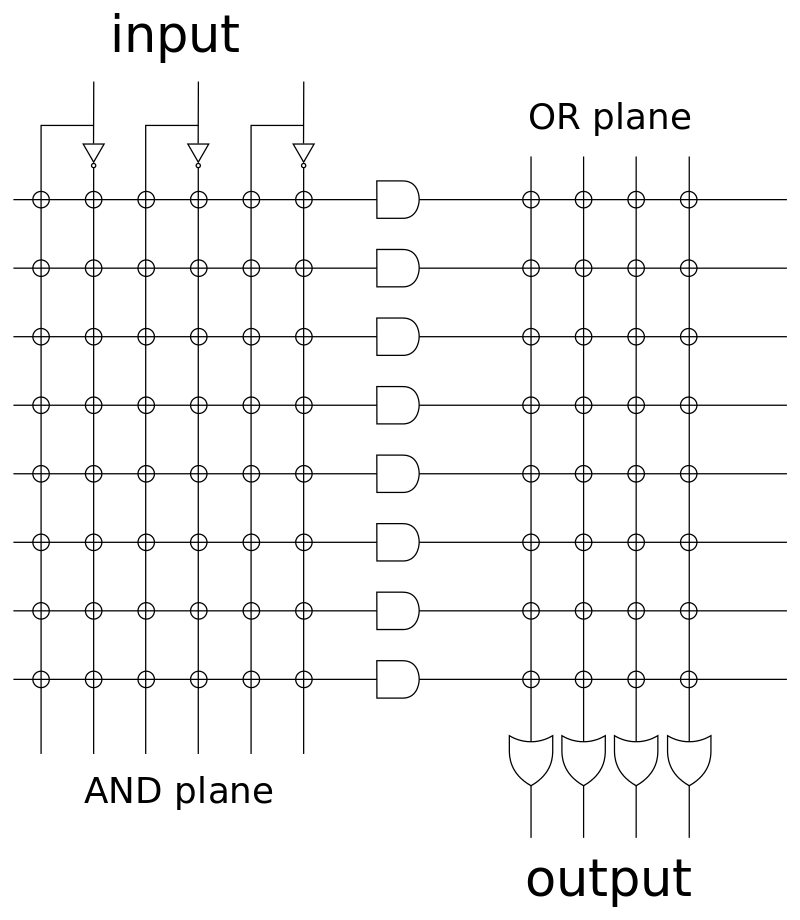
\includegraphics[width=.6\textwidth]{figuras/PLA.png}
\caption{Conexões internas AND e OR de um PLA}
\label{fig:exampleFig1}
\end{figure}

\subsection{\esp Programmable Array Logic (PAL)}
Lógica de Array Programável (PAL) é um circuito integrado semelhante a um PLA (Programmable Logic Arrays) diferenciado pelas portas disponponíveis para programação, sendo a porta AND conectada de acordo com as necessidades do usuário e a porta OR fixa e com o numero de entradas variado.

\begin{figure}[ht]
\centering
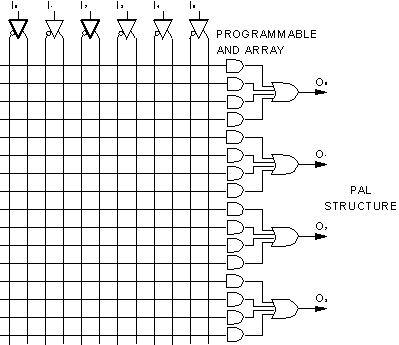
\includegraphics[width=.6\textwidth]{figuras/PAL.png}
\caption{Conexões AND (variáveis) e OR (fixas) de um PAL}
\label{fig:exampleFig2}
\end{figure}



\section{\esp Diferenciação entre CPLDs e FPGAs}

Apesar de serem os principais dispositivos lógicos programáveis utilizados na industria, CPLDs e FPGAs possuem algumas diferenças características que influenciam sua usabilidade.

\subsection{\esp Principais Diferenças}
Uma das principais diferenças entre os dois circuitos integrados é atribuída a sua construção: Enquanto Dispositivos lógicos programáveis complexos (CPLDs) são formados por algumas centenas de blocos lógicos grandes (mais complexos), já Matriz de portas programáveis (FPGAs) são compostos por blocos lógicos mais simples (Flip-Flops) em maior quantidade.

Outra principal diferença observada entre os dois circuitos integrados é o tipo de memória em que se baseiam, sendo FPGAs baseados em RAM, o que faz com que percam sua programação quando a alimentação é cortada enquanto CPLDs são baseados em um tipo de ROM, mantendo sua programação mesmo sem alimentação.

Além disso, no que tange a eficiência e aplicabilidade dos circuitos aponta-se os CPLDs como tendo menor tempo de resposta (mais eficientes) por possuírem uma quandidade menor de plocos lógicos, entretando isso os torna menos flexíveis. No quesito aplicabilidade FPGAs possuem menos restrições, podendo ser aplicados em projetos mais abranjentes e complexos, enquanto CPLDs são limitados à projetos de menor escopo.


\subsection{\esp Diferenças Estruturais}
A principal diferença estrutural entre os circuitos integrados é a quantidade e o tipo dos blocos que integram os circuitos. Observa-se que FPGAs possuem um numero elevado de blocos e conexões enquanto CPLDs possuem blocos maiores e em menor quantidade.



\begin{figure}[ht]
\centering
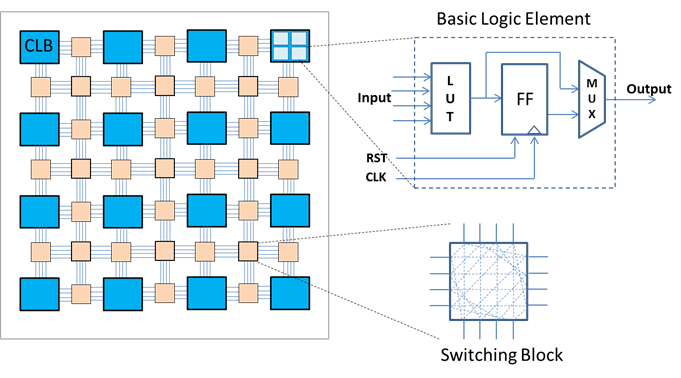
\includegraphics[width=.8\textwidth]{figuras/FPGA_diagram.png}
\caption{Diagrama de conexões de um FPGA}
\label{fig:exampleFig2}
\end{figure}


\begin{figure}[ht]
\centering
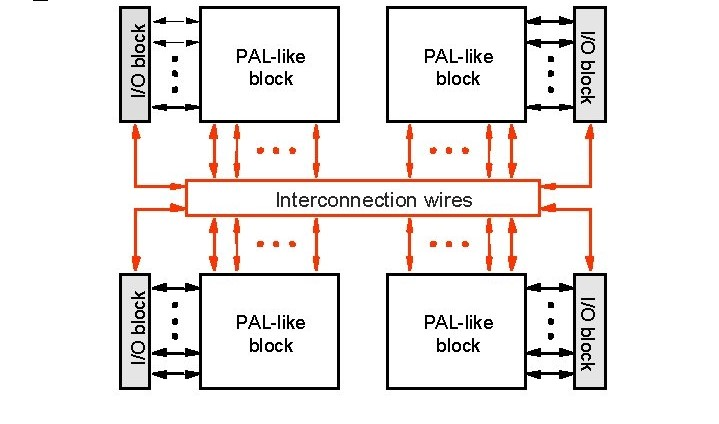
\includegraphics[width=.8\textwidth]{figuras/CPLD.jpg}
\caption{Diagrama de conexões de um CPLD}
\label{fig:exampleFig2}
\end{figure}
   
\section{REFERÊNCIAS}

FREITAS, Tiago Tobias; PASQUALIANOTO, Thiago Luiz; LEÃO, Juliano Carlos Leão.1O CPLD (Dispositivo Complexo de Lógica Programação aplicado em automação industrial. Feira SENAI Paulista de Inovação Tecnológica  -  INOVASENAI, 2005.

O.A.C.Macedo; P.B.Alves;  N.Marranghello. DISPOSITIVOS LÓGICOS PROGRAMÁVEIS. UNIVERSIDADE ESTADUAL PAULISTA, nov. 2002.

DIZ RAMOS, M.L.P; CURI, E. Análise de erro em avaliação de sistemas digitais: uma questão com lógica. REVEMAT, v. 8, ano 2015, p. 16, 26 agosto 2015. Disponível em: <https://periodicos.ufsc.br/index.php/revemat/article/view/1981-1322.2013v8n1p232/25136>. Acesso em: 28 mar. 2022.
 




%%%%%%%%%%%%%%%%%%%%%%%%%%%%%%%%%%%
%% FIM DO TEXTO
%%%%%%%%%%%%%%%%%%%%%%%%%%%%%%%%%%%

% \selectlanguage{brazil}
%%%%%%%%%%%%%%%%%%%%%%%%%%%%%%%%%%%
%% Inicio bibliografia
%%%%%%%%%%%%%%%%%%%%%%%%%%%%%%%%%%%

 \newpage
\singlespace{
\renewcommand\refname{REFERÊNCIAS}
\bibliographystyle{abntex2-alf}
\bibliography{bibliografia}

}

\end{document}


